\documentclass[11pt,psfig]{article}
\usepackage{epsfig}
\usepackage{times}
\usepackage{amssymb}
\usepackage{float}

\newcount\refno\refno=1
\def\ref{\the\refno \global\advance\refno by 1}
\def\ux{\underline{x}}
\def\ut{\underline{\theta}}
\def\umu{\underline{\mu}}
\def\be{p_e^*}
\newcount\eqnumber\eqnumber=1
\def\eq{\the \eqnumber \global\advance\eqnumber by 1}
\def\eqs{\eq}
\def\eqn{\eqno(\eq)}

 \pagestyle{empty}
\def\baselinestretch{1.1}
\topmargin1in \headsep0.3in
\topmargin0in \oddsidemargin0in \textwidth6.5in \textheight8.5in
\begin{document}
\setlength{\parskip}{1.2ex plus0.3ex minus 0.3ex}


\thispagestyle{empty} \pagestyle{myheadings} \markright{Homework
5: CS 274A, Probabilistic Learning: Winter 2014}



\title{CS 274A Homework 5}
\author{Zachary DeStefano, 15247592}
\date{Due Date: Wednesday March 5th}

\maketitle

 \newpage

\section*{K-means plots}

\subsection*{Plots of Clusters}

\begin{figure}[H]
\centering
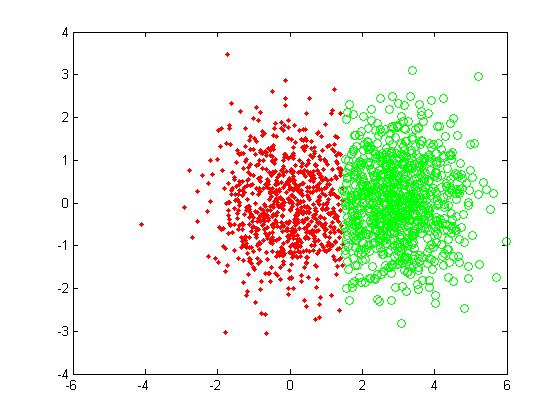
\includegraphics[height=3.25in]{dataset1_kMeansPlot.jpg}
\caption{The k-Means plot for dataset1, K=2}
\end{figure}

\begin{figure}[H]
\centering
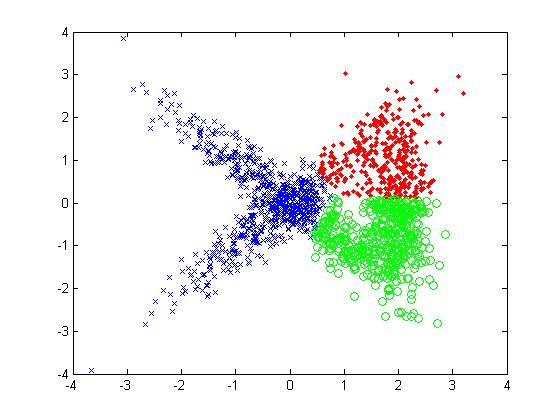
\includegraphics[height=3.25in]{dataset2_kMeansPlot.jpg}
\caption{The k-Means plot for dataset2, K=3}
\end{figure}

\begin{figure}[H]
\centering
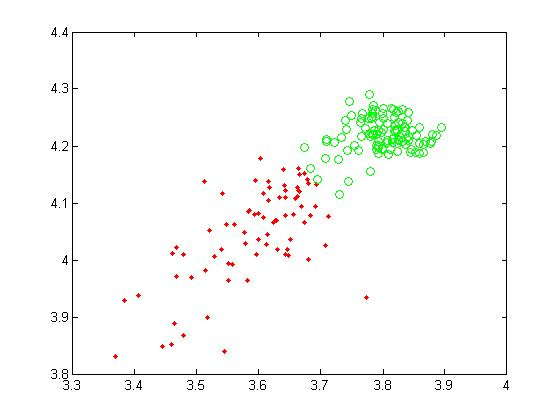
\includegraphics[height=3.25in]{dataset3_kMeansPlot.jpg}
\caption{The k-Means plot for dataset3, K=2}
\end{figure}

\subsection*{Plots of Sum of Squared Errors versus Iteration}

\begin{figure}[H]
\centering
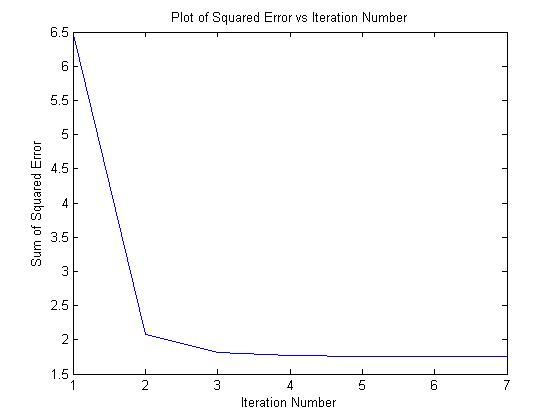
\includegraphics[height=3.25in]{dataset1_kMeans_squaredErrorPlot.jpg}
\caption{The Sum of Squared Error plot for dataset1, K=2}
\end{figure}

\begin{figure}[H]
\centering
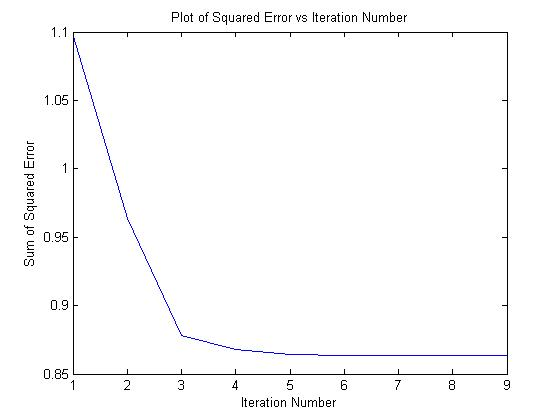
\includegraphics[height=3.25in]{dataset2_kMeans_squaredErrorPlot.jpg}
\caption{The Sum of Squared Error plot for dataset2, K=3}
\end{figure}

\begin{figure}[H]
\centering
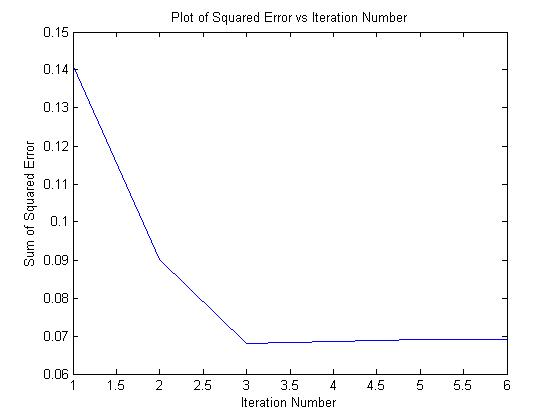
\includegraphics[height=3.25in]{dataset3_kMeans_squaredErrorPlot.jpg}
\caption{The Sum of Squared Error plot for dataset3, K=2}
\end{figure}

\section*{EM plots}

\subsection*{Plots of clusters using EM algorithm}

\begin{figure}[H]
\centering
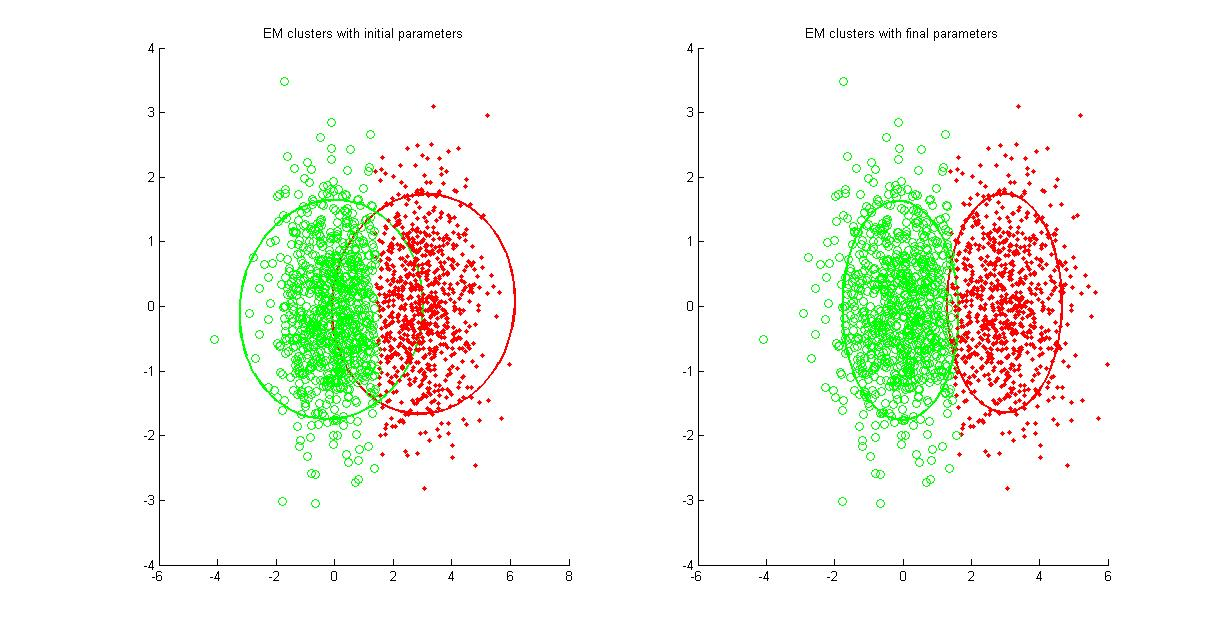
\includegraphics[height=3in]{dataset1_EMclusterPlots.jpg}
\caption{The EM cluster plots for dataset1, K=2}
\end{figure}

\subsection*{Plots of likelihood using EM algorithm}

\begin{figure}[H]
\centering
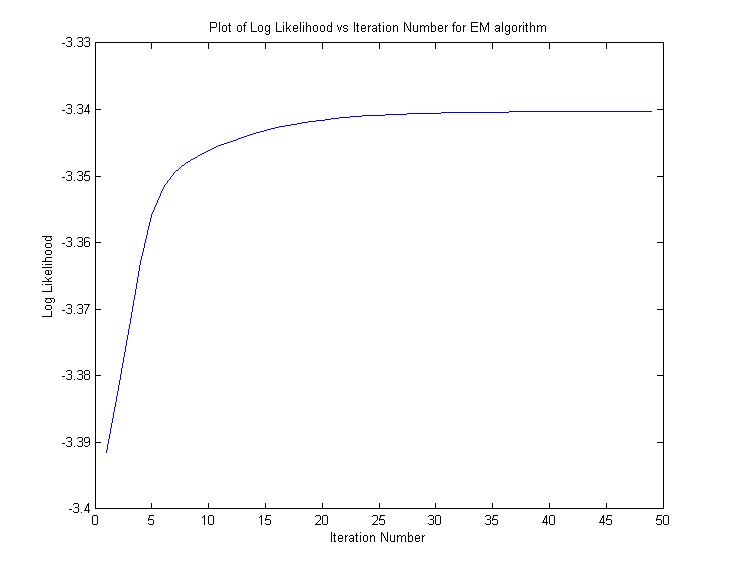
\includegraphics[height=3.25in]{dataset1_EMlogLikelihoodPlot.jpg}
\caption{The likelihood plot for dataset1, K=2}
\end{figure}

\end{document}
